\documentclass{article} 
%All documents start with this
% This is called the preamble. It sets up the format of the document.
% It includes author information, dates, formatting etc.
% If we require any additional formatting etc, we can import ‘packages’.
% This will give us more customability.
% For exmaple: ams* packages gives us a range of symbols etc.
\usepackage{color}
\usepackage{graphicx}
\usepackage{amsmath, amsthm, amsfonts, amssymb}
\usepackage{lipsum}
% fancyhdr is a package that deals with headers and footers.
\usepackage{fancyhdr}
\setlength{\headheight}{15pt}
\pagestyle{fancyplain}
% Header and Footer content
\lhead{\today}
\chead{\LaTeX{} Primer}
\rhead{\thepage}
\lfoot{left footer}
\cfoot{\thepage}
\rfoot{right footer}
% Preamble ends here
\begin{document}

\title{My First Document}
\author{My Name}
\date{\today}
\maketitle

% \pagenumbering{roman}
% \tableofcontents
% \listoffigures
% \listoftables
% \newpage
% \pagenumbering{arabic}


% This is where the content starts, after this line.
\begin{abstract}
  This is the start of a \LaTeX primer....
\end{abstract}

\section{Punctuation Symbols}
\subsection{quotes}
Note the difference in right and left quotes in \lq single
quotes\rq\ and \lq\lq double quotes\rq\rq


\subsection{dashes}
Note that a single dash character in the input - produces a hyphen in the output, two
dashes -- produces a longer dash (--) in the output and three dashes --- produce the
longest dash (---) in the output


\subsection{accents}
\'{E}l est\'{a} aqu\'{\i}


\subsection{special symbols}
Maybe I have now learnt about 1\% of \LaTeX

\textasciitilde; \&; \#; \_; \$; \textbackslash; \%; \{; \}; \textasciicircum



\section{Fonts and Tyles}

\subsection{style}
\textsf{\textbf{sans serif family, boldface series, upright shape}}\\
\textrm{\textsl{roman family, medium series, slanted shape}}\\
\textit{A polygon of three sides is called a \emph{triangle} and a
polygon of four sides is called a \emph{quadrilateral}}

\noindent roman \textrm{roman}\\
sans serif \textsf{sans serif}\\
typewriter \texttt{typewriter}\\
medium \textmd{medium}\\
boldface \textbf{boldface}\\  
upright \textup{upright}\\
italic \textit{italic}\\
slanted \textsl{slanted}\\
SMALL CAP \textsc{small cap}\\


\subsection{size}
size tiny {\tiny size}\\
size scriptsize {\scriptsize size}\\
size footnotesize {\footnotesize size}\\
size small {\small size}\\
size normalsize {\normalsize size}\\
size large {\large size}\\
size Large {\Large size}\\
size LARGE {\LARGE size}\\
size huge {\huge size}\\
size Huge {\Huge size}


\begin{figure}[h]
  \centering
  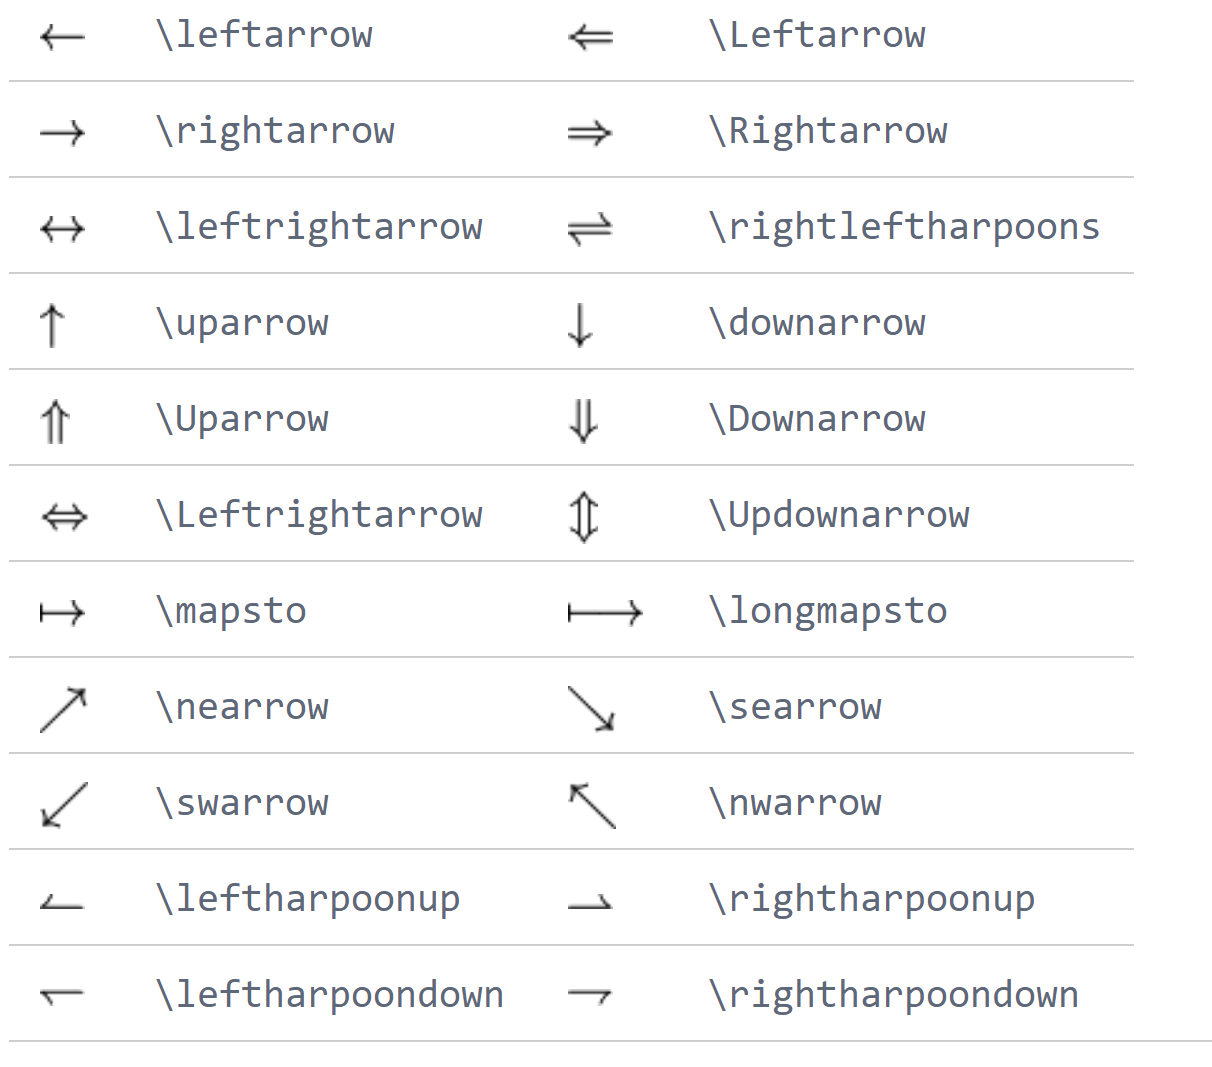
\includegraphics[width=0.5\linewidth]{latex-math-arrows.png}
  \caption{latex page layout sys}
  \label{fig:latex-lmath-arrows}
\end{figure}

% Write all the content here, before this line.
\section{section}
\lipsum[3]
\subsection{subsection}
\lipsum[10]
\subsubsection{subsubsection}
\lipsum[1-2]
\paragraph{paragraph}
\lipsum[2-3]
\subparagraph{subparagraph}
\lipsum[1-2]

\section{Lorem}
\lipsum[1-5]


\end{document}